\documentclass{beamer}
\usetheme[faculty=ped,basePath=../fibeamer,logo=../fibeamer/logo/mu/Logo-UC-3.png]{fibeamer}
\graphicspath{{../resources/}}

\usepackage{algorithm}
\usepackage{algpseudocode}

\usetheme[faculty=ped]{fibeamer}
\usepackage[utf8]{inputenc}
\usepackage[
  main=english,
  czech, slovak
]{babel}
\title{Programación Orientada a Objetos}
\subtitle{Semestre II-2026}
\author{Profesora: Andreina Cota Vidaurre}

\usepackage{ragged2e}
\usepackage{booktabs}
\usepackage{tabularx}
\usepackage{tikz}
\usetikzlibrary{calc, shapes, backgrounds}
\usetikzlibrary{positioning, arrows.meta, shadows.blur, shapes.geometric}
\usepackage{amsmath, amssymb}
\usepackage{url}
\usepackage{listings}
\usepackage{graphicx}
\usepackage{amsmath}
\usepackage[T1]{fontenc}
\usepackage{xcolor}
\usepackage{minted}

\lstdefinelanguage{PseudocodigoES}{
    morekeywords={INICIO,FIN,PARA,HACER,SI,ENTONCES,FIN_SI,FIN_PARA,IMPRIMIR},
    sensitive=true,
    morecomment=[l]{//},
    morestring=[b]"
}

\lstdefinelanguage{PseudocodeEN}{
    morekeywords={BEGIN,END,FOR,DO,IF,THEN,END_IF,END_FOR,PRINT},
    sensitive=true,
    morecomment=[l]{//},
    morestring=[b]"
}

\lstset{
    basicstyle=\ttfamily\small,
    keywordstyle=\bfseries,
    columns=fullflexible,
    keepspaces=true,
    showstringspaces=false,
    frame=single,
    xleftmargin=0em,
    framexleftmargin=0em,
    framesep=2pt,
    gobble=4,
    resetmargins=true,
    aboveskip=0pt,
    belowskip=0pt
}

\lstdefinestyle{pythonstyle}{
    language=Python,
    basicstyle=\ttfamily\small,
    keywordstyle=\bfseries,
    commentstyle=\itshape,
    stringstyle=\ttfamily,
    showstringspaces=false,
    columns=fullflexible,
    keepspaces=true,
    frame=single,
    breaklines=true,
    xleftmargin=0em,
    framexleftmargin=0em,
    framesep=2pt,
    aboveskip=0pt,
    belowskip=0pt,
    gobble=4,
    resetmargins=true,
    emph={print,input,int,float,str,bool,len,range},
    emphstyle=\bfseries
}

\lstset{style=pythonstyle}

\tikzstyle{iniciofin} = [
    ellipse,
    minimum width=2.5cm,
    minimum height=1cm,
    text centered,
    draw=black,
    fill=blue!25
]

\tikzstyle{proceso} = [
    rectangle,
    rounded corners,
    minimum width=3cm,
    minimum height=1cm,
    text centered,
    draw=black,
    fill=cyan!20
]

\tikzstyle{decision} = [
    diamond,
    aspect=2,
    text centered,
    draw=black,
    fill=yellow!35
]

\tikzstyle{flecha} = [
    thick,
    ->,
    >=Stealth
]

\frenchspacing
\begin{document}
  \shorthandoff{-}
  \frame[c]{\maketitle}

    %------------------------------------------------------------------
    \begin{frame}{Contenido}
        \begin{itemize}
            \item Motivación: de las listas a los objetos.
            \item Programación Orientada a Objetos: clases y objetos.
            \item Definición de clases: \mintinline{python}{class}, \mintinline{python}{__init__} y \mintinline{python}{self}.
            \item Atributos y creación de objetos.
            \item Métodos y representación textual con \mintinline{python}{__str__}.
            \item Relaciones e interacción entre objetos.
            \item Ejercicios de aplicación.
            \item Síntesis.
        \end{itemize}
    \end{frame}
    
    % ----------------------------------------------------------------
    % BLOQUE 1: MOTIVACIÓN
    % ----------------------------------------------------------------
    \begin{frame}{Motivación}
        \textcolor{blue}{\textbf{¿Cómo representarías una colección de canciones en Python?}}
    
        \vspace{1em}
        Cada canción tiene un título, un artista y una duración.
    
        \vspace{1em}
        \begin{itemize}
            \item ¿Qué estructuras de datos conocemos para almacenar esta información?
            \pause
            \item ¿Cómo accederíamos a la duración de una canción?
            \pause
            \item ¿Cómo calcularíamos la duración total de varias canciones?
        \end{itemize}
    \end{frame}
    
    \begin{frame}[fragile,t]{Motivación: usando listas}
        Podemos representar canciones con listas:
        \begin{minted}[xleftmargin=-2cm, frame=leftline, fontsize=\small]{python}
            cancion1 = ["Gracias a la vida", "Violeta Parra", 273]
            cancion2 = ["Tren al sur", "Los Prisioneros", 328]
    
            canciones = [cancion1, cancion2]
            print(canciones[0][2])  # Duración de la primera canción
        \end{minted}
        \pause
        \textcolor{blue}{\textbf{Para discutir:}}
        \begin{itemize}
            \item ¿Qué significa el índice \texttt{2}?
            \item ¿Qué ocurriría si cambiamos el orden de los datos?
            \item ¿Cómo nos aseguramos de que todas las canciones tengan la misma estructura?
        \end{itemize}
    \end{frame}
    
    \begin{frame}[fragile,t]{Motivación: datos y operaciones}
        También podemos definir funciones que trabajen con esos datos:
        \begin{minted}[xleftmargin=-2cm, frame=leftline, fontsize=\small]{python}
            def duracion_minutos(cancion):
                return cancion[2] / 60
            
            print(duracion_minutos(cancion1))
        \end{minted}
        \pause
        \begin{itemize}
            \item Los datos y las operaciones se definen por separado.
            \item El código debe conocer qué representa cada posición.
            \item Las listas y las funciones siguen siendo útiles, pero podemos organizar el programa de otra manera.
        \end{itemize}
        \vspace{0.3em}
        \textcolor{blue}{\textbf{¿Podemos reunir los datos de una canción y las operaciones asociadas?}}
    \end{frame}
    
    % ----------------------------------------------------------------
    % BLOQUE 2: CLASES Y OBJETOS
    % ----------------------------------------------------------------
    \begin{frame}{Programación Orientada a Objetos (POO)}
        \textbf{POO} es un paradigma de programación que modela un problema como un conjunto de \textbf{objetos}
        que interactúan entre sí.
        \pause
        \vspace{0.8em}

        Ejemplo: una canción reúne datos y operaciones en un mismo modelo.
        \renewcommand{\arraystretch}{1.35}
        \begin{center}
            \footnotesize
            \begin{tabular}{@{}p{4.8cm}p{5.2cm}@{}}
                \toprule
                \textbf{Datos (atributos)} & \textbf{Operaciones (métodos)} \\
                \midrule
                Título & Obtener duración en minutos \\
                Artista & Generar una descripción \\
                Duración & \\
                \bottomrule
            \end{tabular}
        \end{center}
    \end{frame}
    
    \begin{frame}{Clase y Objeto}
        \begin{itemize}
            \item \textbf{Clase:} Abstracción que representa un tipo de entidad a partir de sus características esenciales: 
            \begin{itemize}
                \item \textcolor{blue}{Estado}. Descrito mediante atributos.
                \item \textcolor{cyan}{Comportamiento}. Definido mediante métodos. 
            \end{itemize}
            La clase describe \textcolor{blue}{cómo es} y \textcolor{cyan}{qué puede hacer} esa entidad, sin referirse a ningún caso particular.
            \pause
            \item \textbf{Objeto:} Instancia concreta de una clase que tiene \textcolor{blue}{atributos}, 
            que determinan su estado, y puede ejecutar los \textcolor{cyan}{métodos} definidos por su clase.
            \vspace{0.5em}

            Dos objetos de una misma clase comparten estructura y comportamiento, pero son entidades distintas e independientes.
        \end{itemize}
    \end{frame}

    \begin{frame}{Clase y Objeto}
        \begin{figure}
            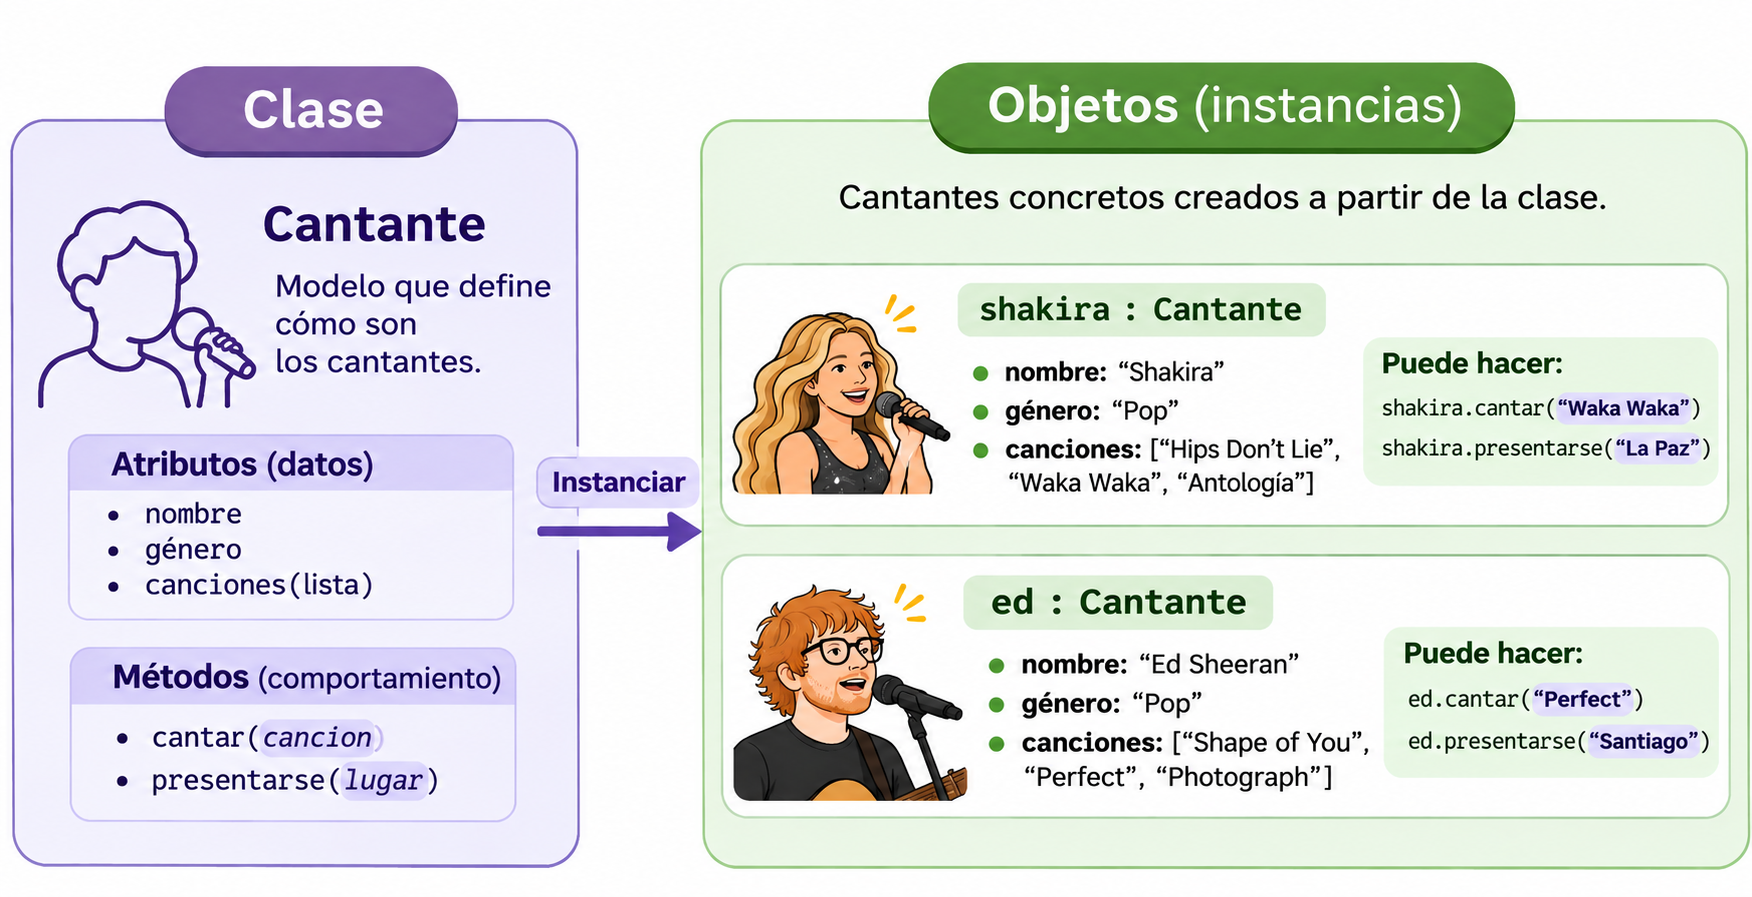
\includegraphics[width=\textwidth]{cantante.png}
        \end{figure}
    \end{frame}
    
    \begin{frame}{¿Qué elementos definen una clase?}
        \begin{itemize}
            \item \textbf{Atributos:} Datos que describen el estado de un objeto.
            \pause
            \item \textbf{Métodos:} Operaciones que pueden realizarse sobre un objeto.
        \end{itemize}
        % \vspace{0.5em}
        % \begin{center}
        %     \begin{tabular}{|l|}
        %         \hline
        %         \multicolumn{1}{|c|}{\textbf{Cancion}} \\ \hline
        %         titulo \\
        %         artista \\
        %         duracion \\ \hline
        %         duracion\_minutos() \\
        %         descripcion() \\ \hline
        %     \end{tabular}
        % \end{center}
        \begin{figure}
            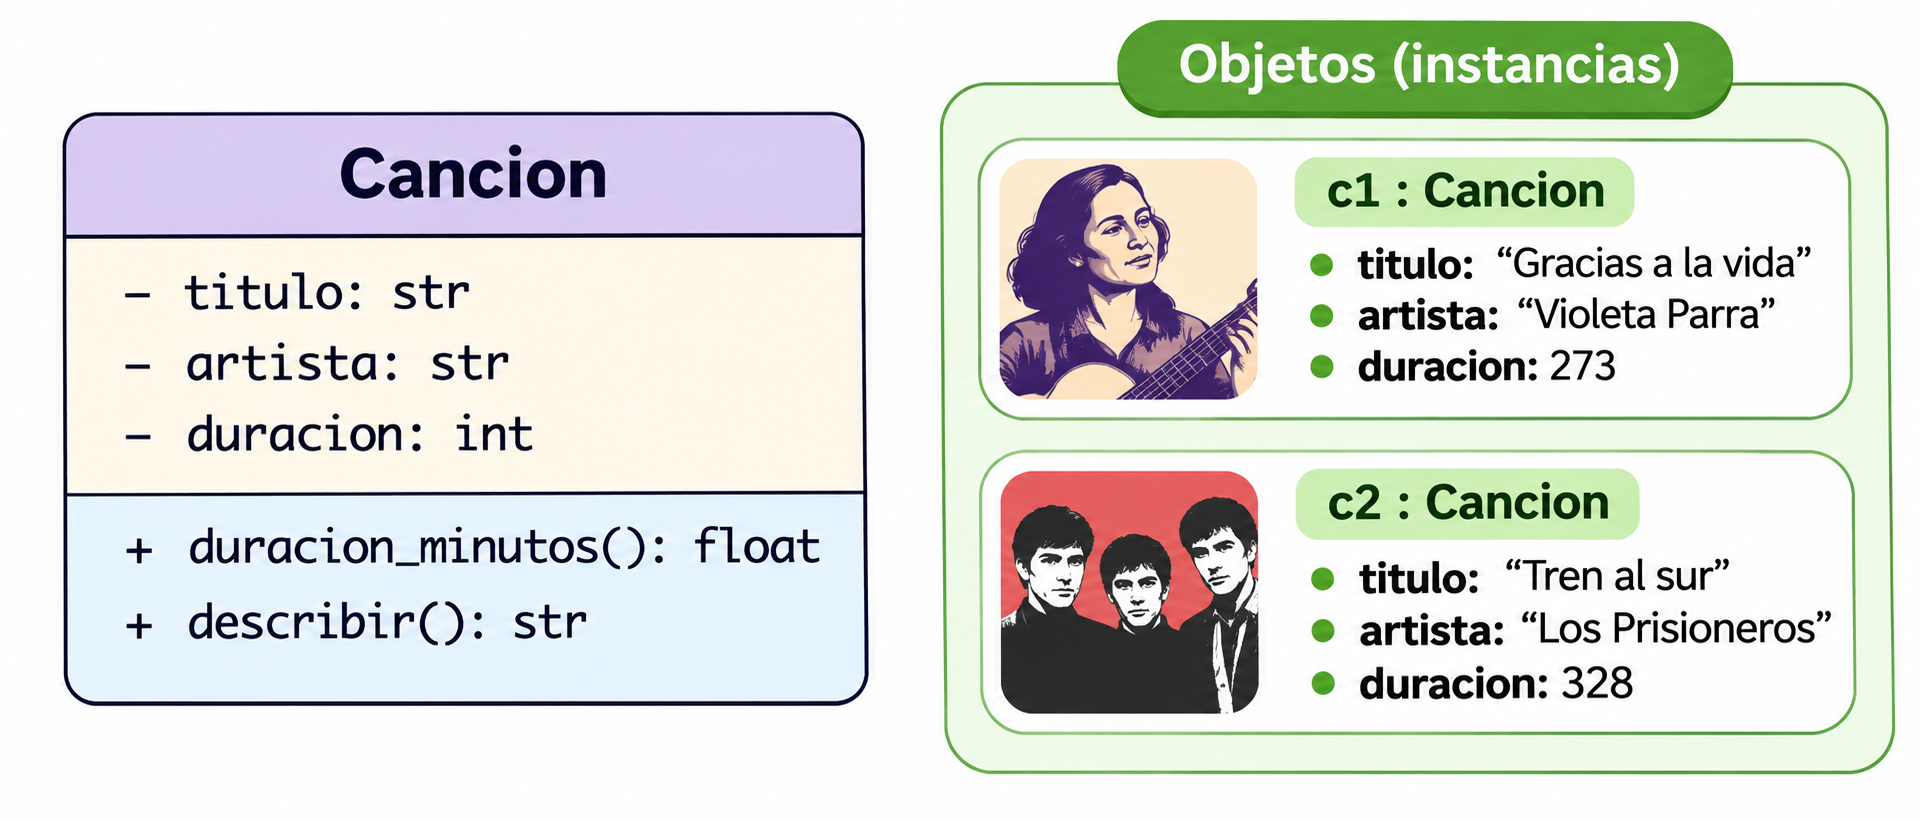
\includegraphics[width=\textwidth]{cancion.png}
        \end{figure}
    \end{frame}
    
    % ----------------------------------------------------------------
    % BLOQUE 3: DEFINICIÓN E INSTANCIACIÓN
    % ----------------------------------------------------------------
    \begin{frame}[fragile,t]{Definición de una clase en Python}
        En Python, una clase se define con \mintinline{python}{class}:
        \begin{minted}[xleftmargin=-2cm, frame=leftline, fontsize=\small]{python}
            class Cancion:
                def __init__(self, titulo, artista, duracion):
                    self.titulo = titulo
                    self.artista = artista
                    self.duracion = duracion
        \end{minted}
        \pause
        \begin{itemize}
            \item \mintinline{python}{class} introduce la definición de una clase.
            \item \mintinline{python}{__init__} inicializa una nueva instancia.
            \item Los parámetros reciben los valores iniciales.
            \item Los nombres de clases suelen escribirse en \textbf{PascalCase}: \mintinline{python}{Cancion}, 
            \mintinline{python}{Estudiante}, \mintinline{python}{IntroProgramacion}.
        \end{itemize}
    \end{frame}
    
    \begin{frame}[fragile,t]{Inicialización de objetos: \texttt{self}}
        Consideremos la siguiente instrucción:
        \begin{minted}[xleftmargin=-2cm, frame=leftline, fontsize=\small]{python}
            cancion1 = Cancion("Gracias a la vida", "Violeta Parra", 273)
        \end{minted}
        Dentro de \mintinline{python}{__init__} se ejecutan asignaciones como:
        \begin{minted}[xleftmargin=-2cm, frame=leftline, fontsize=\small]{python}
            self.titulo = titulo
        \end{minted}
        \pause
        \begin{itemize}
            \item \mintinline{python}{titulo}: Parámetro que recibe un valor.
            \item \mintinline{python}{self.titulo}: Atributo de la instancia.
            \item \mintinline{python}{self}: Referencia al objeto que se está inicializando o usando.
        \end{itemize}
    \end{frame}

    \begin{frame}{Inicialización de objetos}
        \begin{figure}
            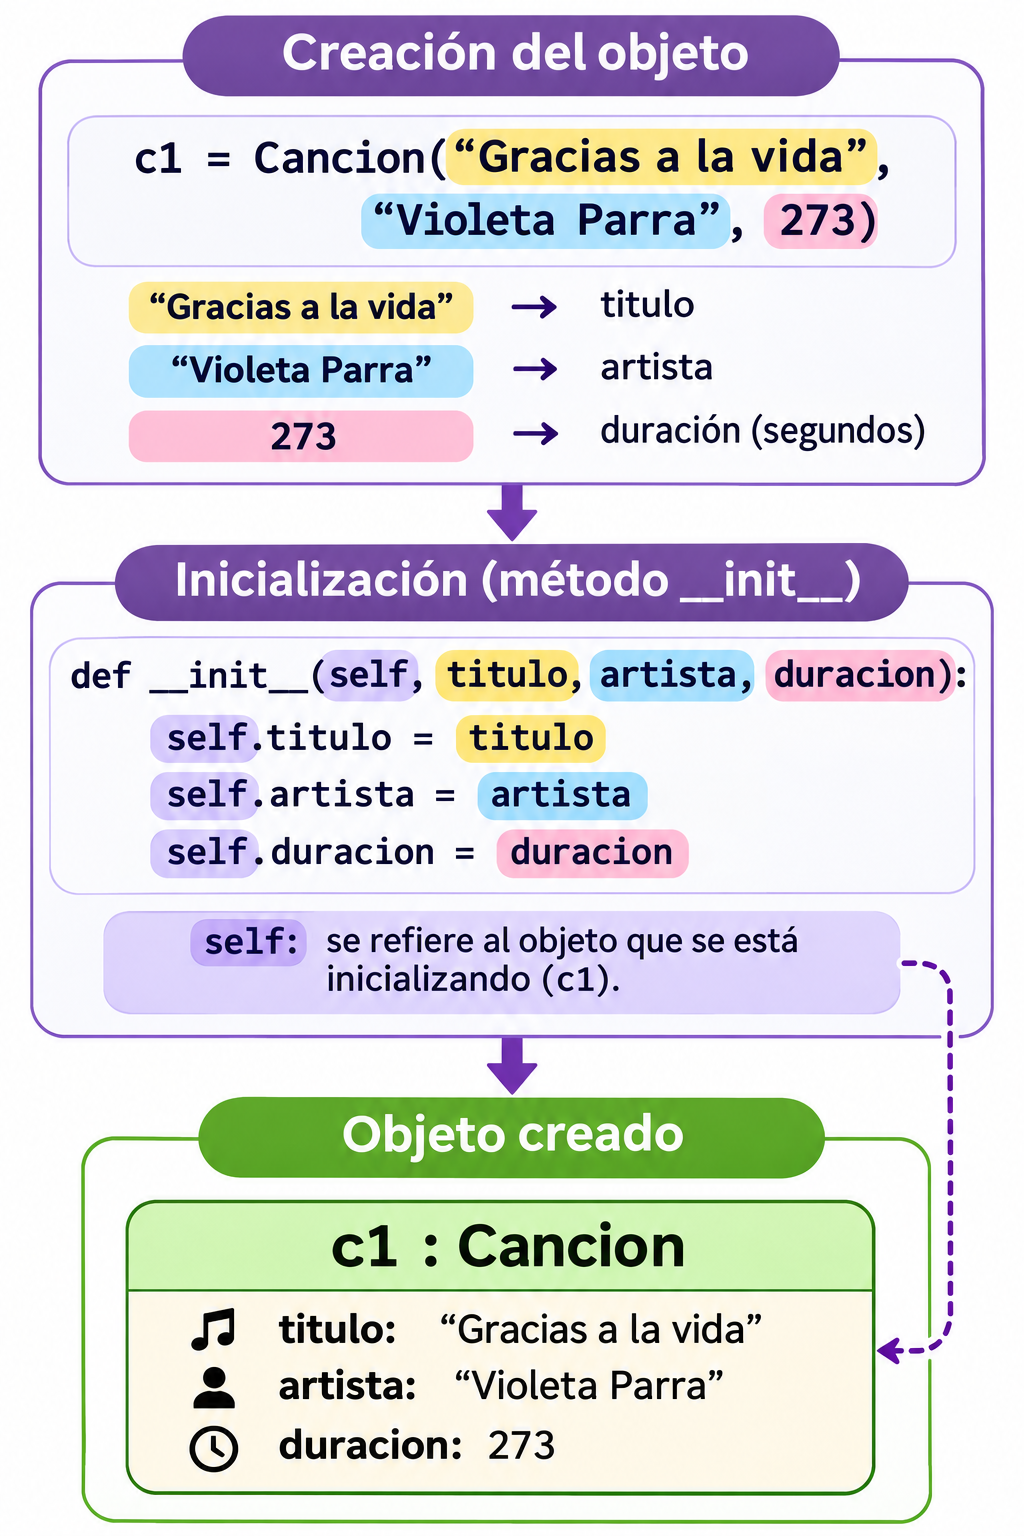
\includegraphics[width=0.48\textwidth]{inicializacion_2.png}
        \end{figure}
    \end{frame}
    
    \begin{frame}[fragile,t]{Creación de objetos}
        Una vez definida la clase, podemos crear distintas instancias:
        \begin{minted}[xleftmargin=-2cm, frame=leftline, fontsize=\small]{python}
            cancion1 = Cancion("Gracias a la vida", "Violeta Parra", 273)
            cancion2 = Cancion("Tren al sur", "Los Prisioneros", 328)
        \end{minted}
        \pause
        \begin{itemize}
            \item Ambas instancias pertenecen a la clase \mintinline{python}{Cancion}.
            \item Cada una almacena sus propios valores.
            \item La variable \mintinline{python}{cancion1} hace referencia a un objeto distinto de \mintinline{python}{cancion2}.
        \end{itemize}
        % REUTILIZAR IMAGEN 1: Resaltar ahora las variables cancion1 y cancion2.
        \textcolor{blue}{\textbf{Pregunta:}} si cambia la duración de \mintinline{python}{cancion1}, ¿cambia también la de \mintinline{python}{cancion2}?
    \end{frame}
    
    \begin{frame}[fragile,t]{Acceso y modificación de atributos}
        La \textbf{notación punto} permite acceder a los atributos:
        \begin{minted}[xleftmargin=-2cm, frame=leftline, fontsize=\small]{python}
            print(cancion1.titulo)
            print(cancion1.duracion)
            
            cancion1.duracion = 275
            print(cancion1.duracion)
        \end{minted}
        \pause
        \textbf{Sintaxis:} \mintinline{python}{objeto.atributo}
        \vspace{0.5em}

        Cada objeto conserva sus propios valores, que pueden consultarse o modificarse cuando corresponda.
    \end{frame}
    
    \begin{frame}[fragile,t]{Actividad: ¿cuál es la salida?}
        \begin{minted}[xleftmargin=-2cm, frame=leftline, fontsize=\small]{python}
            a = Cancion("Canción A", "Artista 1", 180)
            b = Cancion("Canción B", "Artista 2", 240)
            
            a.duracion = 200
            
            print(a.duracion)
            print(b.duracion)
        \end{minted}
        \pause
        \textcolor{blue}{\textbf{¿Qué valores se mostrarán?}}

        \pause
        \textbf{Respuesta:} \mintinline{python}{200} y \mintinline{python}{240}
    \end{frame}

    \begin{frame}[fragile,t]{Métodos: comportamiento de los objetos}
        ¿Cómo calcular la duración de \textbf{una canción} en minutos?
        \begin{minted}[xleftmargin=-2cm, frame=leftline, fontsize=\small]{python}
            def duracion_minutos(segundos):
                return segundos / 60
        \end{minted}
        \pause
        Como \textbf{método de instancia}, la operación utiliza un atributo del objeto:
        \begin{minted}[xleftmargin=-2cm, frame=leftline, fontsize=\small]{python}
            def duracion_minutos(self):
                return self.duracion / 60
        \end{minted}
        \pause
        \begin{minted}[xleftmargin=-2cm, frame=leftline, fontsize=\small]{python}
            print(cancion1.duracion_minutos())
        \end{minted}
        % IMAGEN SUGERIDA 4: Comparar funcion(datos) con objeto.metodo().
    \end{frame}
    
    \begin{frame}[fragile,t]{Métodos: una clase completa}
        El método se define dentro de la clase:
        \begin{minted}[xleftmargin=-2cm, frame=leftline, fontsize=\small]{python}
            class Cancion:
                def __init__(self, titulo, artista, duracion):
                    self.titulo = titulo
                    self.artista = artista
                    self.duracion = duracion
            
                def duracion_minutos(self):
                    return self.duracion / 60
            
            c = Cancion("Gracias a la vida", "Violeta Parra", 273)
            print(c.duracion_minutos())
        \end{minted}
    \end{frame}
    
    \begin{frame}[fragile,t]{Representación textual: \mintinline{python}{__str__}}
        ¿Qué sucede al imprimir directamente un objeto?
        \begin{minted}[xleftmargin=-2cm, frame=leftline, fontsize=\small]{python}
            print(c)
            # Sin __str__, se obtiene una representación como:
            # <__main__.Cancion object at 0x...>
        \end{minted}
        \pause
        Podemos definir una representación más comprensible:
        \begin{minted}[xleftmargin=-2cm, frame=leftline, fontsize=\small]{python}
            # Añadir dentro de la clase Cancion
            def __str__(self):
                return self.titulo + " - " + self.artista
                \end{minted}
                \pause
                \begin{minted}[xleftmargin=-2cm, frame=leftline, fontsize=\small]{python}
            print(c)  # Gracias a la vida - Violeta Parra
        \end{minted}
        \begin{itemize}
            \item \mintinline{python}{__str__} debe retornar una cadena de caracteres.
            \item Se utiliza mediante \mintinline{python}{print(objeto)} o \mintinline{python}{str(objeto)}.
        \end{itemize}
    \end{frame}
    
    \begin{frame}[fragile,t]{Métodos que utilizan otros métodos}
        Un método puede llamar a otro del mismo objeto mediante \mintinline{python}{self}:
        \begin{minted}[xleftmargin=-2cm, frame=leftline, fontsize=\small]{python}
            # Dentro de la clase Cancion
            def duracion_minutos(self):
                return self.duracion / 60
            
            def descripcion(self):
                return self.titulo + ": " + \
                    str(round(self.duracion_minutos(), 2)) + " min"
        \end{minted}
        \pause
        \begin{minted}[xleftmargin=-2cm, frame=leftline, fontsize=\small]{python}
            print(c.descripcion())
        \end{minted}
        \textbf{Idea clave:} \mintinline{python}{self.duracion_minutos()} ejecuta un método del mismo objeto.
    \end{frame}
    
    % ----------------------------------------------------------------
    % BLOQUE 5: RELACIONES E INTERACCIÓN
    % ----------------------------------------------------------------
    \begin{frame}[fragile,t]{Listas de objetos}
        Una lista puede almacenar objetos de una clase:
        \begin{minted}[xleftmargin=-2cm, frame=leftline, fontsize=\small]{python}
            canciones = [
                Cancion("Gracias a la vida", "Violeta Parra", 273),
                Cancion("Tren al sur", "Los Prisioneros", 328)
            ]
            
            print(canciones[0].titulo)
            
            for cancion in canciones:
                print(cancion.titulo)
        \end{minted}
        \pause
        \textcolor{blue}{¿Y si la lista de reproducción también necesita un nombre y sus propios métodos?}
    \end{frame}

    \begin{frame}{Listas de objetos}
        \begin{figure}
            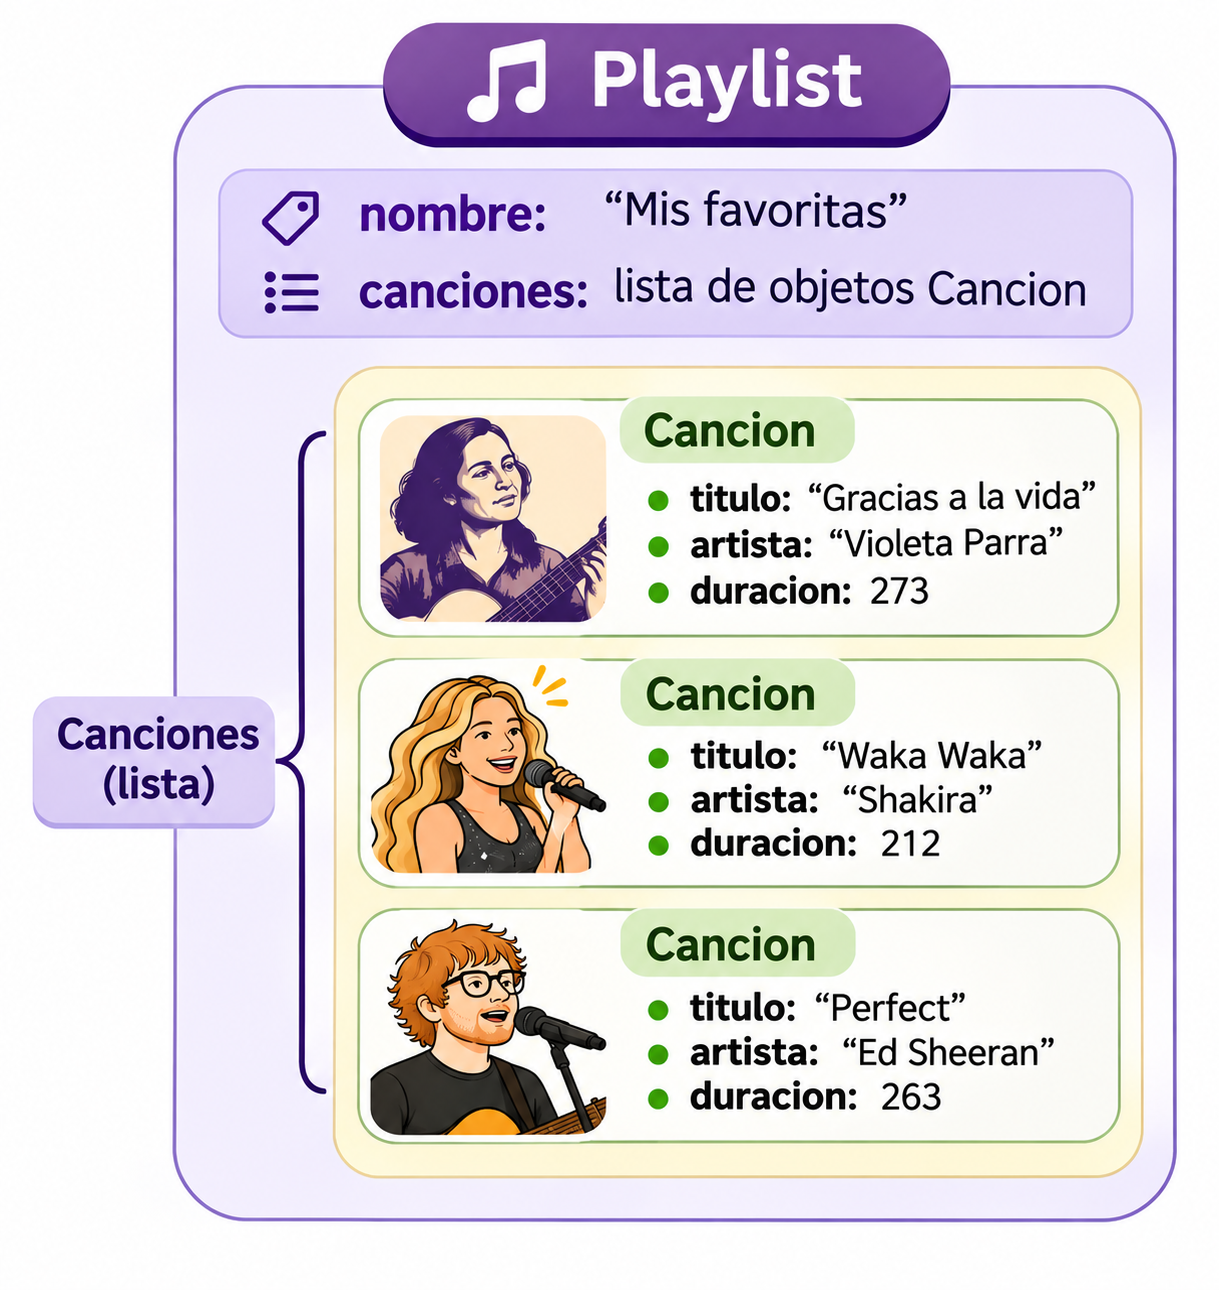
\includegraphics[width=0.7\textwidth]{playlist.png}
        \end{figure}
    \end{frame}
    
    \begin{frame}[fragile,t]{Objetos que contienen listas de objetos}
        Podemos definir una clase \mintinline{python}{Playlist} que almacene canciones:
        \begin{minted}[xleftmargin=-2cm, frame=leftline, fontsize=\small]{python}
            class Playlist:
                def __init__(self, nombre):
                    self.nombre = nombre
                    self.canciones = []
            
                def agregar(self, cancion):
                    self.canciones.append(cancion)
        \end{minted}
        \pause

        \begin{minted}[xleftmargin=-2cm, frame=leftline, fontsize=\small]{python}
            lista = Playlist("Mis favoritas")
            c1 = Cancion("Gracias a la vida", "Violeta Parra", 273)
            lista.agregar(c1)
        \end{minted}
        % IMAGEN SUGERIDA 5: Tarjeta Playlist con atributo canciones.
        % Flechas desde la lista hacia tarjetas de objetos Cancion.
        Un atributo puede almacenar una lista de referencias a otros objetos.
    \end{frame}
    
    \begin{frame}[fragile,t]{Interacción entre objetos}
        La \texttt{Playlist} puede usar los atributos de las canciones que almacena:
        \begin{minted}[xleftmargin=-2cm, frame=leftline, fontsize=\small]{python}
            # Dentro de la clase Playlist
            def total_segundos(self):
                total = 0
                for cancion in self.canciones:
                    total += cancion.duracion
                return total
        \end{minted}
        \pause
        \begin{itemize}
            \item El objeto \texttt{Playlist} recorre otros objetos.
            \item Accede a \mintinline{python}{cancion.duracion} en cada instancia.
            \item Utiliza esos valores para calcular su propio resultado.
        \end{itemize}
    \end{frame}
    
    \begin{frame}[fragile,t]{Interacción: llamar métodos de otros objetos}
        Los objetos también pueden utilizar los \textbf{métodos} de otros objetos:
        \begin{minted}[xleftmargin=-2cm, frame=leftline, fontsize=\small]{python}
            # Dentro de la clase Playlist
            def total_minutos(self):
                total = 0
                for cancion in self.canciones:
                    total += cancion.duracion_minutos()
                return total
                \end{minted}
        \pause
        \textbf{Diferencia importante:}\\
        \mintinline{python}{self.total_minutos()} llama a un método de la \texttt{Playlist};\\
        \mintinline{python}{cancion.duracion_minutos()} llama a un método de cada \texttt{Cancion}.
        % IMAGEN SUGERIDA 6: Playlist -> Cancion A / Cancion B;
        % cada Cancion retorna minutos -> Playlist acumula los resultados.
    \end{frame}
    
    \begin{frame}[fragile,t]{Ejemplo integrado: usar los objetos}
        Suponiendo definidas las clases \mintinline{python}{Cancion} y \mintinline{python}{Playlist} con sus métodos:
        \begin{minted}[xleftmargin=-2cm, frame=leftline, fontsize=\small]{python}
            lista = Playlist("Mis favoritas")
            
            c1 = Cancion("Gracias a la vida", "Violeta Parra", 273)
            c2 = Cancion("Tren al sur", "Los Prisioneros", 328)
            
            lista.agregar(c1)
            lista.agregar(c2)
            
            print(lista.nombre)
            print(lista.total_minutos())
        \end{minted}
    \end{frame}
    
    \begin{frame}[fragile,t]{Objetos que contienen otros objetos}
        Un atributo también puede referirse directamente a otro objeto:
        \begin{minted}[xleftmargin=-2cm, frame=leftline, fontsize=\small]{python}
            class Usuario:
                def __init__(self, nombre):
                    self.nombre = nombre
                    self.playlist = Playlist("Mis favoritas")
            
            usuario = Usuario("Camila")
            c1 = Cancion("Gracias a la vida", "Violeta Parra", 273)
            usuario.playlist.agregar(c1)
        \end{minted}
        \pause
        \begin{itemize}
            \item \mintinline{python}{Usuario} contiene una referencia a una \mintinline{python}{Playlist}.
            \item Esa \mintinline{python}{Playlist} contiene una lista de canciones.
            \item El constructor de \mintinline{python}{Usuario} crea una \mintinline{python}{Playlist} nueva.
        \end{itemize}
        % DIAGRAMA OPCIONAL: Usuario -> Playlist -> [Cancion, Cancion, ...]
    \end{frame}
    
    % ----------------------------------------------------------------
    % BLOQUE 6: EJERCICIOS
    % ----------------------------------------------------------------
    % \begin{frame}{Ejercicios de aplicación}
    %     \begin{enumerate}
    %         \item \textbf{Diseño (sin código):} identificar atributos y métodos de un personaje de videojuego.
    %         \item \textbf{Completar código:} clase \mintinline{python}{Estudiante}, atributos y métodos.
    %         \item \textbf{Relacionar objetos:} clase \mintinline{python}{Curso} con una lista de estudiantes.
    %         \item \textbf{Desafío integrador:} diseñar e implementar pedidos de delivery.
    %     \end{enumerate}
    % \end{frame}
    
    \begin{frame}{Ejercicio 1: Diseñar una clase}
        Un videojuego necesita representar personajes que pueden desplazarse y recibir daño.
        
        \begin{enumerate}
            \item Proponer un nombre para la clase.
            \item Identificar al menos tres atributos.
            \item Proponer dos métodos.
            \item Describir dos objetos distintos de esa clase.
        \end{enumerate}
    \end{frame}
    
    \begin{frame}[fragile,t]{Ejercicio 2: Completar una clase}
        \begin{minted}[xleftmargin=-2cm, frame=leftline, fontsize=\small]{python}
            class Estudiante:
                def __________(self, nombre, id, promedio):
                    self.nombre = __________
                    self.id = id
                    self.__________ = promedio
            
                def __________(self):
                    return self.nombre + " (" + str(self.id) + ")"
            
                def aprobo(self):
                    return self.promedio >= 4.0
            
            e = Estudiante("Camila", 20261234, 5.2)
            print(e)
            print(e.aprobo())
        \end{minted}
    \end{frame}
    
    \begin{frame}[fragile,t]{Ejercicio 2: Solución}
        \begin{minted}[xleftmargin=-2cm, frame=leftline, fontsize=\small]{python}
            class Estudiante:
                def __init__(self, nombre, id, promedio):
                    self.nombre = nombre
                    self.id = id
                    self.promedio = promedio
            
                def __str__(self):
                    return self.nombre + " (" + str(self.id) + ")"
            
                def aprobo(self):
                    return self.promedio >= 4.0
            
            e = Estudiante("Camila", 20261234, 5.2)
            print(e)           # Camila (20261234)
            print(e.aprobo())  # True
        \end{minted}
    \end{frame}
    
    \begin{frame}[fragile,t]{Ejercicio 3: Un curso con estudiantes}
        Un curso tiene un nombre y una lista de objetos \mintinline{python}{Estudiante}.
        \begin{minted}[xleftmargin=-2cm, frame=leftline, fontsize=\scriptsize]{python}
                class Curso:
                    def __init__(self, nombre):
                        self.nombre = nombre
                        self.estudiantes = __________
                
                    def agregar(self, estudiante):
                        self.__________.append(estudiante)
                
                    def cantidad(self):
                        return len(self.estudiantes)
                
                    def promedio_curso(self):
                        if self.cantidad() == 0:
                            return 0
                        suma = 0
                        for e in self.estudiantes:
                            suma += e.__________
                        return suma / self.cantidad()
        \end{minted}
    \end{frame}
    
    \begin{frame}[fragile,t]{Ejercicio 3: Solución y prueba}
        \begin{minted}[xleftmargin=-2cm, frame=leftline, fontsize=\scriptsize]{python}
                class Curso:
                    def __init__(self, nombre):
                        self.nombre = nombre
                        self.estudiantes = []
                
                    def agregar(self, estudiante):
                        self.estudiantes.append(estudiante)
                
                    def cantidad(self):
                        return len(self.estudiantes)
                
                    def promedio_curso(self):
                        if self.cantidad() == 0:
                            return 0
                        suma = 0
                        for e in self.estudiantes:
                            suma += e.promedio
                        return suma / self.cantidad()
        \end{minted}
    \end{frame}
    
    \begin{frame}[fragile,t]{Ejercicio 3: Uso de las clases}
        \begin{minted}[xleftmargin=-2cm, frame=leftline, fontsize=\small]{python}
            ip = Curso("Introducción a la Programación")
            ip.agregar(Estudiante("Camila", 20261234, 5.2))
            ip.agregar(Estudiante("Matías", 20264567, 3.8))
            
            print(ip.cantidad())       # 2
            print(ip.promedio_curso()) # 4.5
        \end{minted}
        \pause


        \begin{itemize}
            \item ¿Qué objeto contiene la lista de estudiantes?
            \item ¿Qué métodos interactúan con otros objetos?
            \item ¿Por qué \mintinline{python}{promedio_curso()} llama a \mintinline{python}{cantidad()} usando \mintinline{python}{self}?
        \end{itemize}
    \end{frame}
    
    \begin{frame}{Ejercicio 4: Pedidos de delivery}
        Una aplicación necesita gestionar pedidos de comida.
        \begin{itemize}
            \item Cada producto tiene un nombre y un precio.
            \item Cada pedido pertenece a un cliente y contiene productos.
            \item Se deben poder agregar productos y calcular el total del pedido.
            \item Al imprimir el pedido, debe mostrarse el cliente y el total.
        \end{itemize}
    \end{frame}
    
    \begin{frame}{Ejercicio 4: diseño propuesto}
        \begin{columns}[T]
            \begin{column}{0.47\textwidth}
                \textbf{Producto}
                \begin{itemize}
                    \item \textbf{Atributos:} nombre, precio
                    \item \textbf{Método:} \mintinline{python}{__str__()}
                \end{itemize}
            \end{column}
            \begin{column}{0.49\textwidth}
                \textbf{Pedido}
                \begin{itemize}
                    \item \textbf{Atributos:} cliente, productos
                    \item \textbf{Métodos:} \mintinline{python}{agregar()}, \mintinline{python}{total()}, \mintinline{python}{__str__()}
                \end{itemize}
            \end{column}
        \end{columns}
    \end{frame}
    
    \begin{frame}[fragile,t]{Ejercicio 4: Solución (Producto)}
        \begin{minted}[xleftmargin=-2cm, frame=leftline, fontsize=\small]{python}
            class Producto:
                def __init__(self, nombre, precio):
                    self.nombre = nombre
                    self.precio = precio
            
                def __str__(self):
                    return self.nombre + ": $" + str(self.precio)
            
            completo = Producto("Completo italiano", 2500)
            bebida = Producto("Bebida", 1200)
            print(completo)
        \end{minted}
    \end{frame}
    
    \begin{frame}[fragile,t]{Ejercicio 4: Solución (Pedido)}
        \begin{minted}[xleftmargin=-2cm, frame=leftline, fontsize=\scriptsize]{python}
                class Pedido:
                    def __init__(self, cliente):
                        self.cliente = cliente
                        self.productos = []
                
                    def agregar(self, producto):
                        self.productos.append(producto)
                
                    def total(self):
                        suma = 0
                        for producto in self.productos:
                            suma += producto.precio
                        return suma
                
                    def __str__(self):
                        return "Pedido de " + self.cliente + \
                            " - total: $" + str(self.total())
        \end{minted}
    \end{frame}
    
    \begin{frame}[fragile,t]{Ejercicio 4: Solución (Pedido)}
        \begin{minted}[xleftmargin=-2cm, frame=leftline, fontsize=\small]{python}
            pedido = Pedido("Valentina")
            pedido.agregar(Producto("Completo italiano", 2500))
            pedido.agregar(Producto("Bebida", 1200))
            
            print(pedido)
            # Pedido de Valentina - total: $3700
            
            print(pedido.total())
            # 3700
        \end{minted}
        \pause
        ¿Qué ocurre cuando \mintinline{python}{print(pedido)} llama a \mintinline{python}{__str__} y este usa \mintinline{python}{self.total()}?
    \end{frame}
    
    % ----------------------------------------------------------------
    % CIERRE
    % ----------------------------------------------------------------
    \begin{frame}{Errores frecuentes}
        \begin{itemize}
            \item \textbf{Confundir clase y objeto:} una clase describe un tipo; un objeto es una instancia concreta.
            \pause
            \item \textbf{Confundir parámetro y atributo:} \mintinline{python}{nombre} no es lo mismo que \mintinline{python}{self.nombre}.
            \pause
            \item \textbf{Omitir \mintinline{python}{self}:} los métodos de instancia lo reciben como primer parámetro convencional.
            \pause
            \item \textbf{Olvidar los paréntesis:} \mintinline{python}{objeto.metodo()} ejecuta el método; \mintinline{python}{objeto.metodo} solo lo referencia.
            \pause
            \item \textbf{Retornar otro tipo en \mintinline{python}{__str__}:} este método debe retornar un \mintinline{python}{str}.
        \end{itemize}
    \end{frame}
    
    \begin{frame}{Síntesis: Programación Orientada a Objetos}
        \begin{itemize}
            \item Una \textbf{clase} define atributos y métodos comunes.
            \pause
            \item Cada \textbf{objeto} es una instancia con sus propios valores.
            \pause
            \item \mintinline{python}{__init__} inicializa; \mintinline{python}{self} identifica la instancia sobre la que se trabaja.
            \pause
            \item Los \textbf{métodos} operan sobre objetos; \mintinline{python}{__str__} define su representación textual.
            \pause
            \item Los objetos pueden \textbf{contener y utilizar otros objetos} para resolver tareas.
        \end{itemize}
    \end{frame}

\end{document}
